\chapter{研究設計與實作}
\indent
Garbage Collection 在處理沒有依據特性分開擺放的資料時,所需的動作較多、時間較長,所造成的壽命損耗也比較多。
如圖\ref{f3.1}所示,灰色為無效資料,打勾的方塊為有效資料,若此時需要 2 個 Block 儲存,則需執行下列動作,才可完成 Garbage Collection:

\begin{itemize}
    \item 複製 Block 1 與 Block 2 中的有效資料
    \item 將有效資料寫入到 Block 3
    \item 清空 Block 1 與 Block 2
\end{itemize}

\begin{figure}[H]
    \centering
    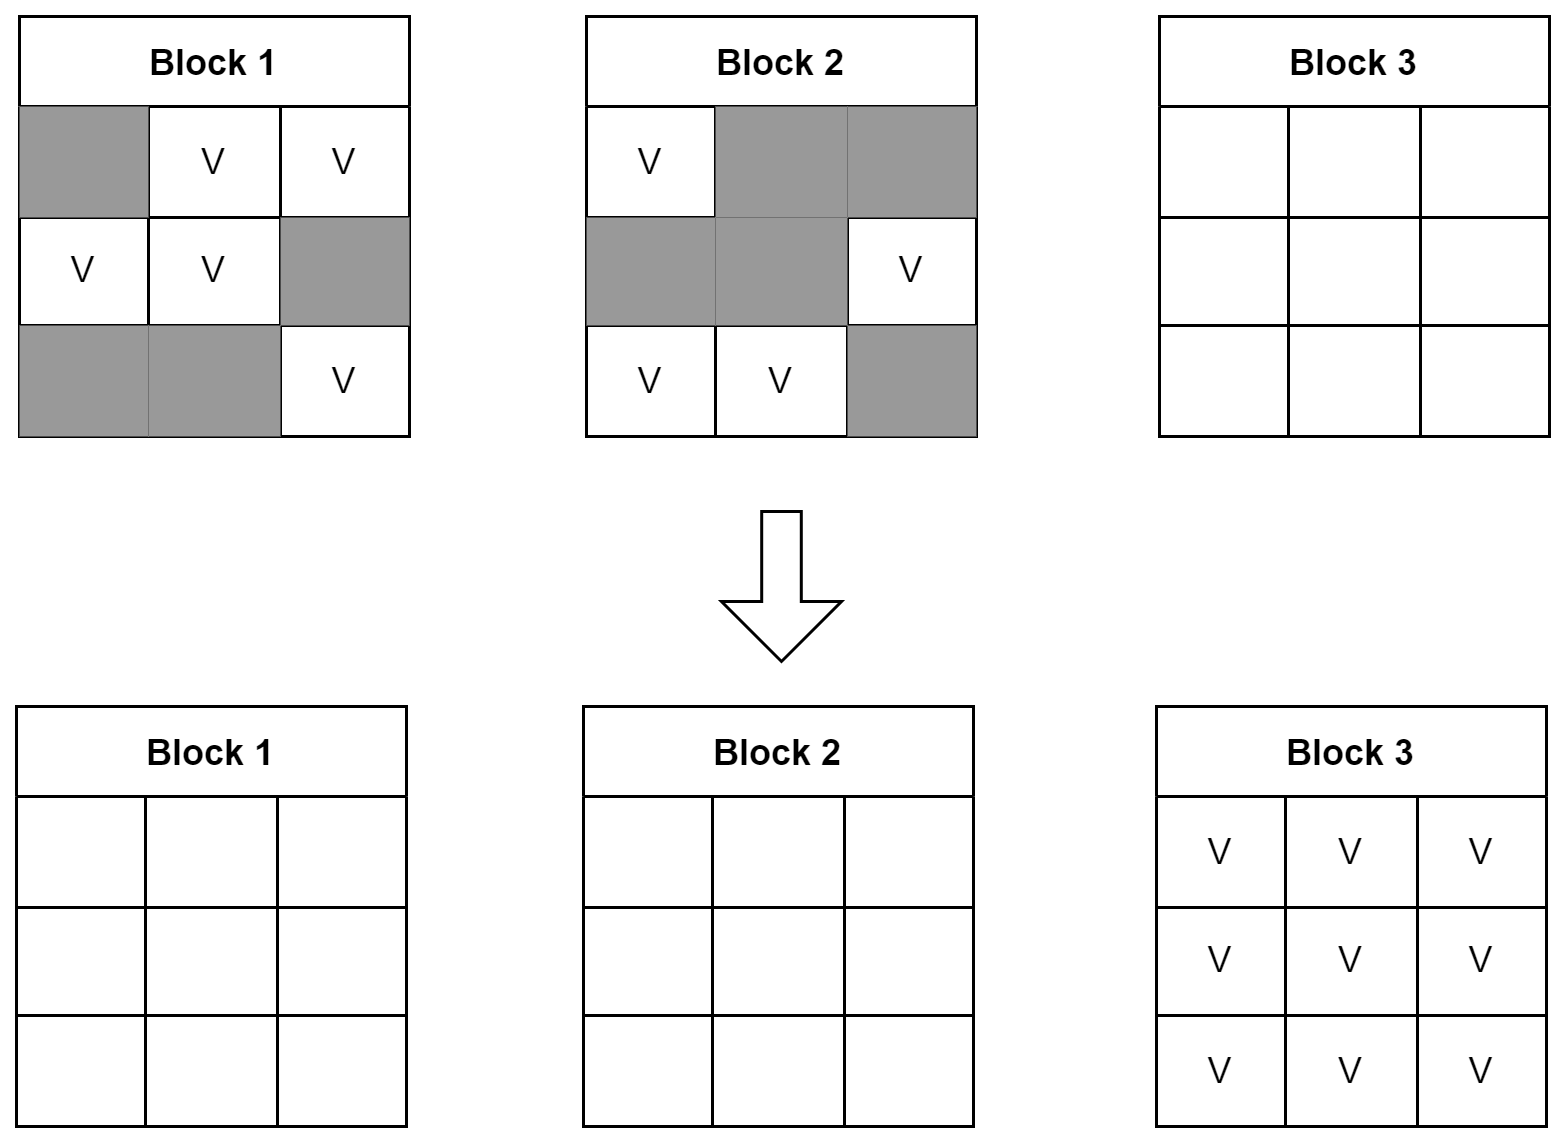
\includegraphics[width=0.8\textwidth]{picture/ch3/gc_efficiency_1.png}
    \caption{Garbage Collection 處理未分群資料}
    \label{f3.1}
\end{figure}

\newpage
\indent
而 Garbage Collection 在處理有依據特性分開擺放的資料時,所需的動作較少、時間較短,所造成的壽命損耗也比較少。
如圖\ref{f3.2}所示,灰色為無效資料,打勾的方塊為有效資料,若此時需要 2 個 Block 儲存,只需執行下列動作,即可完成 Garbage Collection:

\begin{itemize}
    \item 清空 Block 1
\end{itemize}

\begin{figure}[H]
    \centering
    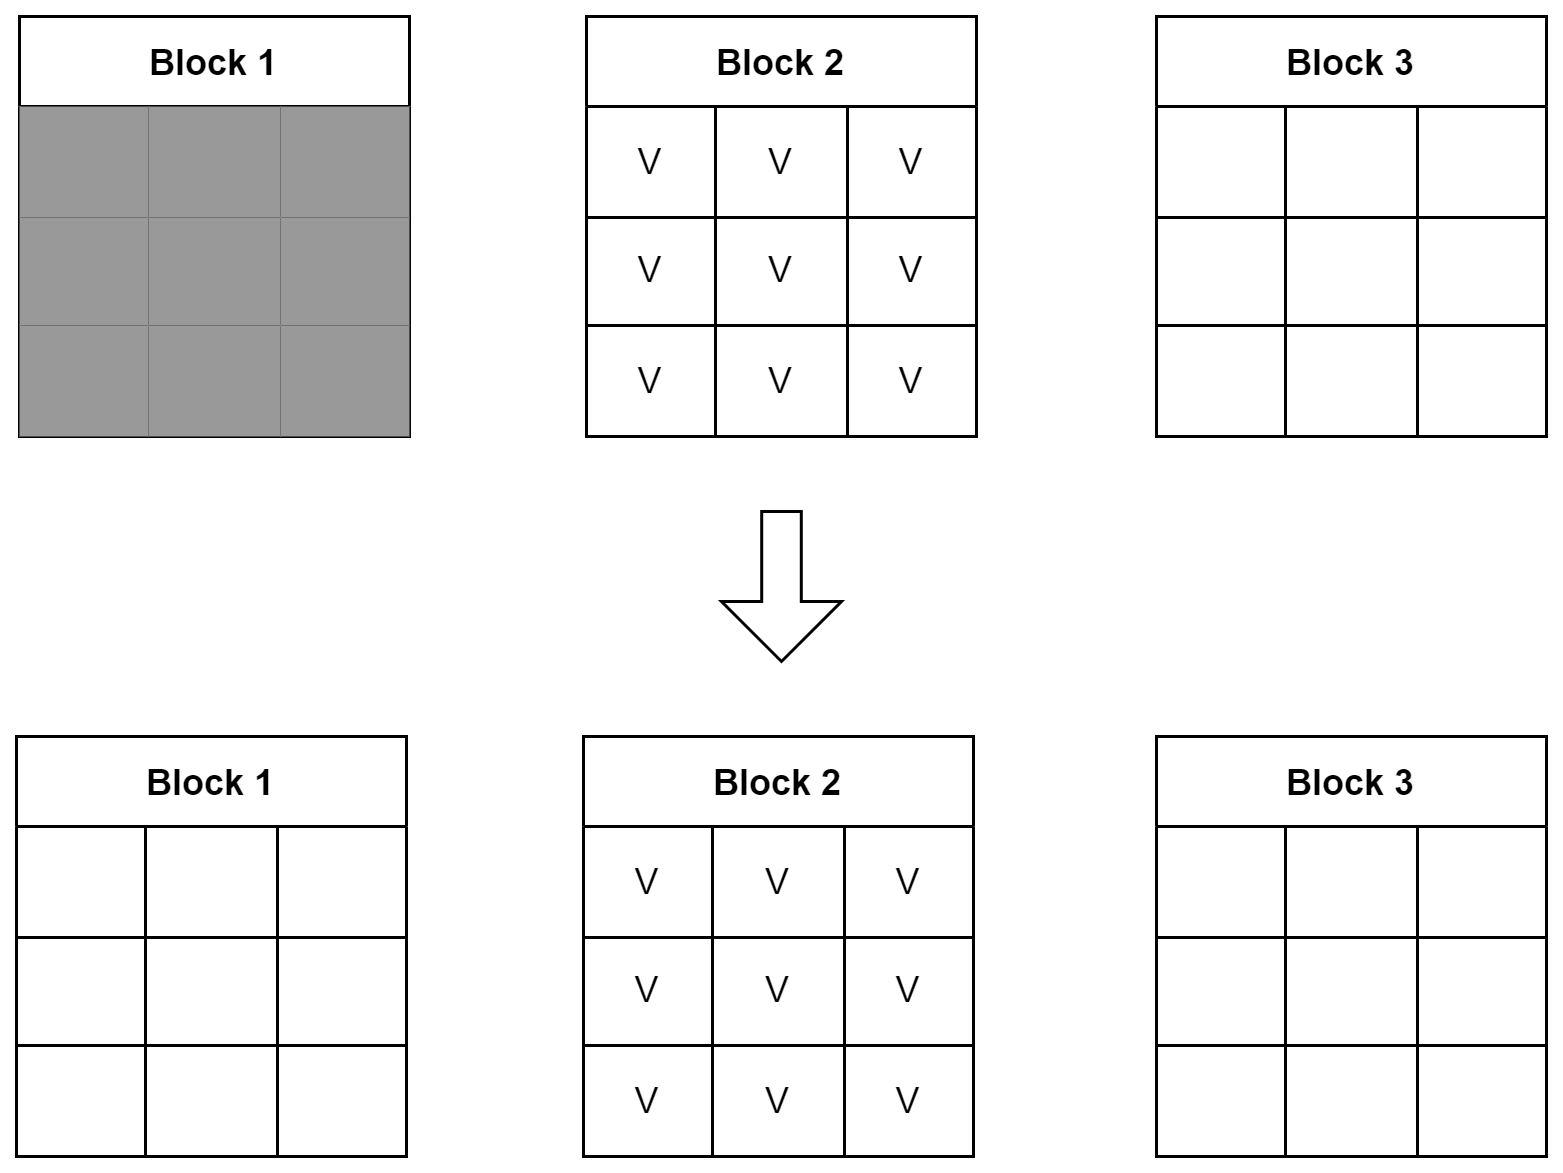
\includegraphics[width=0.8\textwidth]{picture/ch3/gc_efficiency_2.png}
    \caption{Garbage Collection 處理有分群資料}
    \label{f3.2}
\end{figure}

\indent
因此,本論文為提升 Garbage Collection 的效率,以及降低 Garbage Collection 的次數,而提出此設計(如圖\ref{f3.3}所示)。將資料依據熱門到冷門的程度分開擺放,而熱門資料有可能較快被視為無效資料,而因為各自集中的關係,Garbage Collection 所需的動作變少,影響範圍也變小,效率也因此提升。
\begin{figure}[H]
    \centering
    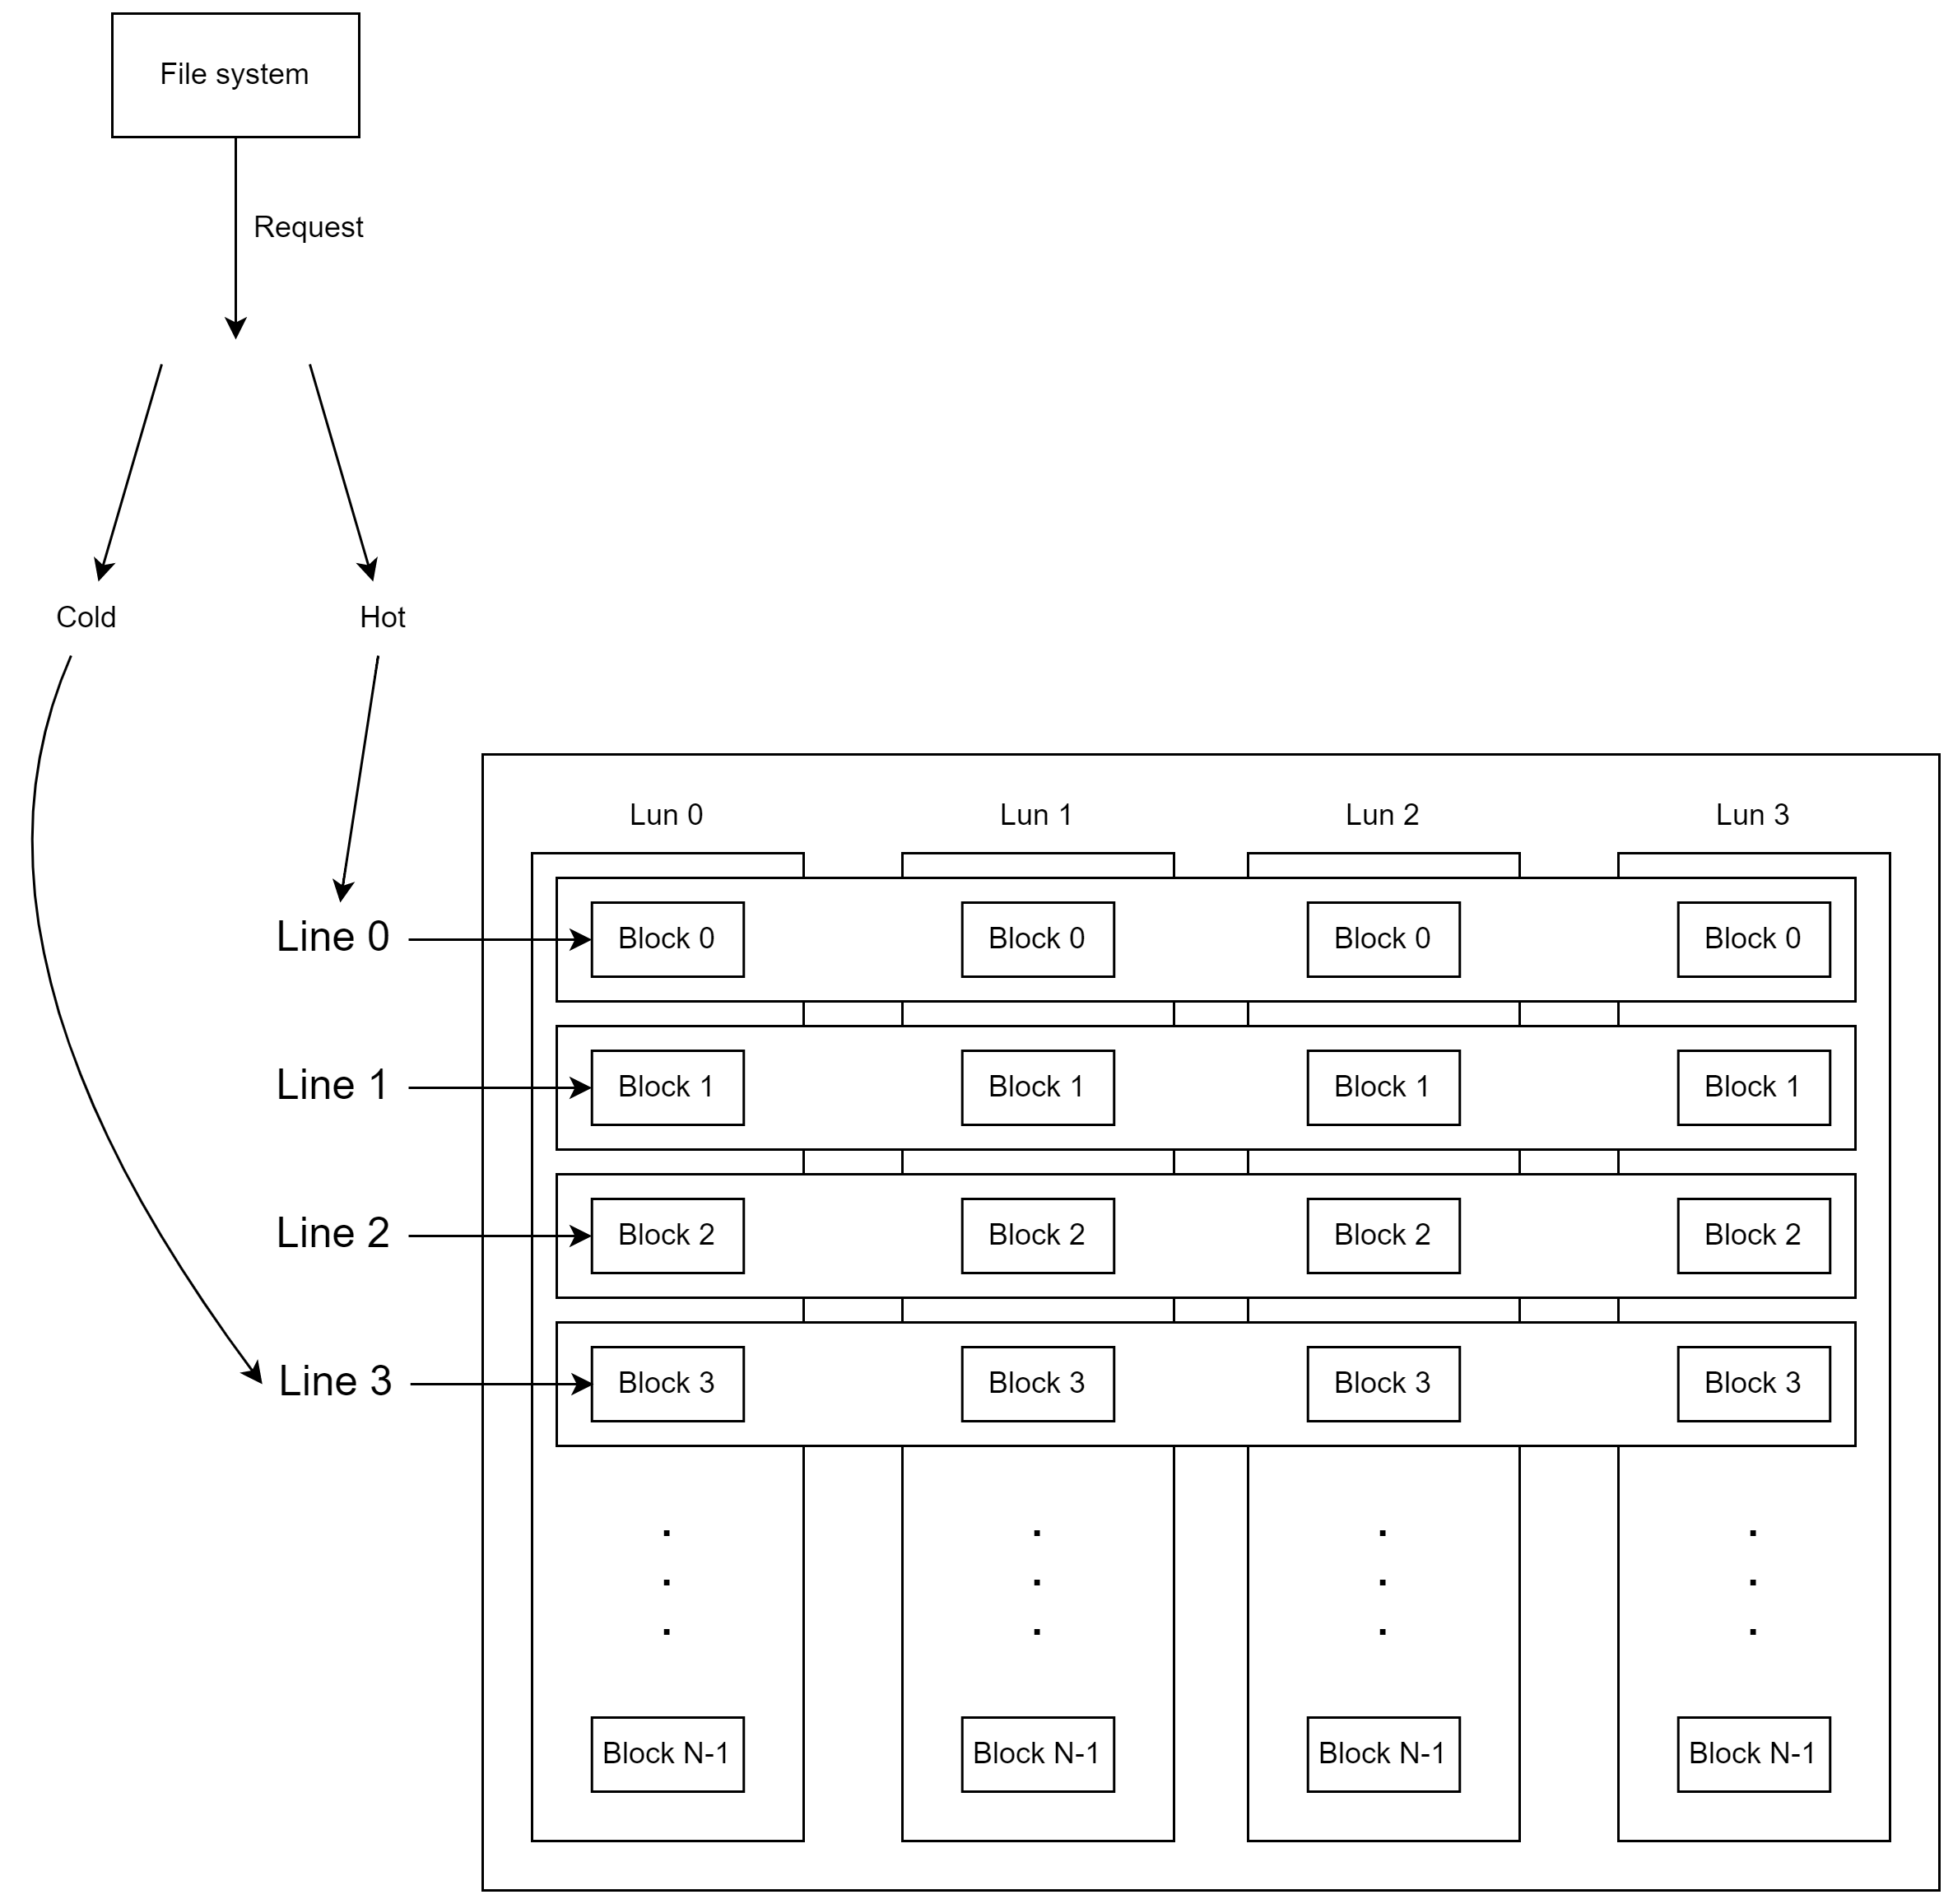
\includegraphics[width=1\textwidth]{picture/ch3/method_3.png}
    \caption{設計方法}
    \label{f3.3}
\end{figure}

透過將此方法與 LightNVM 既有的寫入流程結合,如此一來,LightNVM 在寫入時,會透過這個方法挑選寫入位置,以達成提升效率的目的。\\
\indent
修改大致可分為三部分,第一部分為初始化,讓原本 LightNVM 從準備一個 Line 變成準備四個 Line,一部分為 LightNVM 處理檔案系統的 Request,將資料存入 Ring Buffer;另一部分為 LightNVM 的 Write Thread 會被喚醒,檢查 Ring Buffer 並將 Entry 中紀錄的資料取出,寫到真正的SSD之中,本章節會解釋修改這三部分的哪些環節。

\section{初始化時修改為準備四個 Line}\label{s3.1}
\indent
在初始化時,LightNVM 會先準備好一個 Line,後續有檔案系統傳遞給 LightNVM 寫入要求時,就會從這個 Line 開始寫入,滿了之後會繼續挑選下一個有空間的 Line 來使用,因此我們為了將資料分開寫入,要修改為在初始化時先準備好四個 Line,以便之後的寫入分群使用(如圖\ref{f3.4}所示)。

\begin{figure}[H]
    \centering
    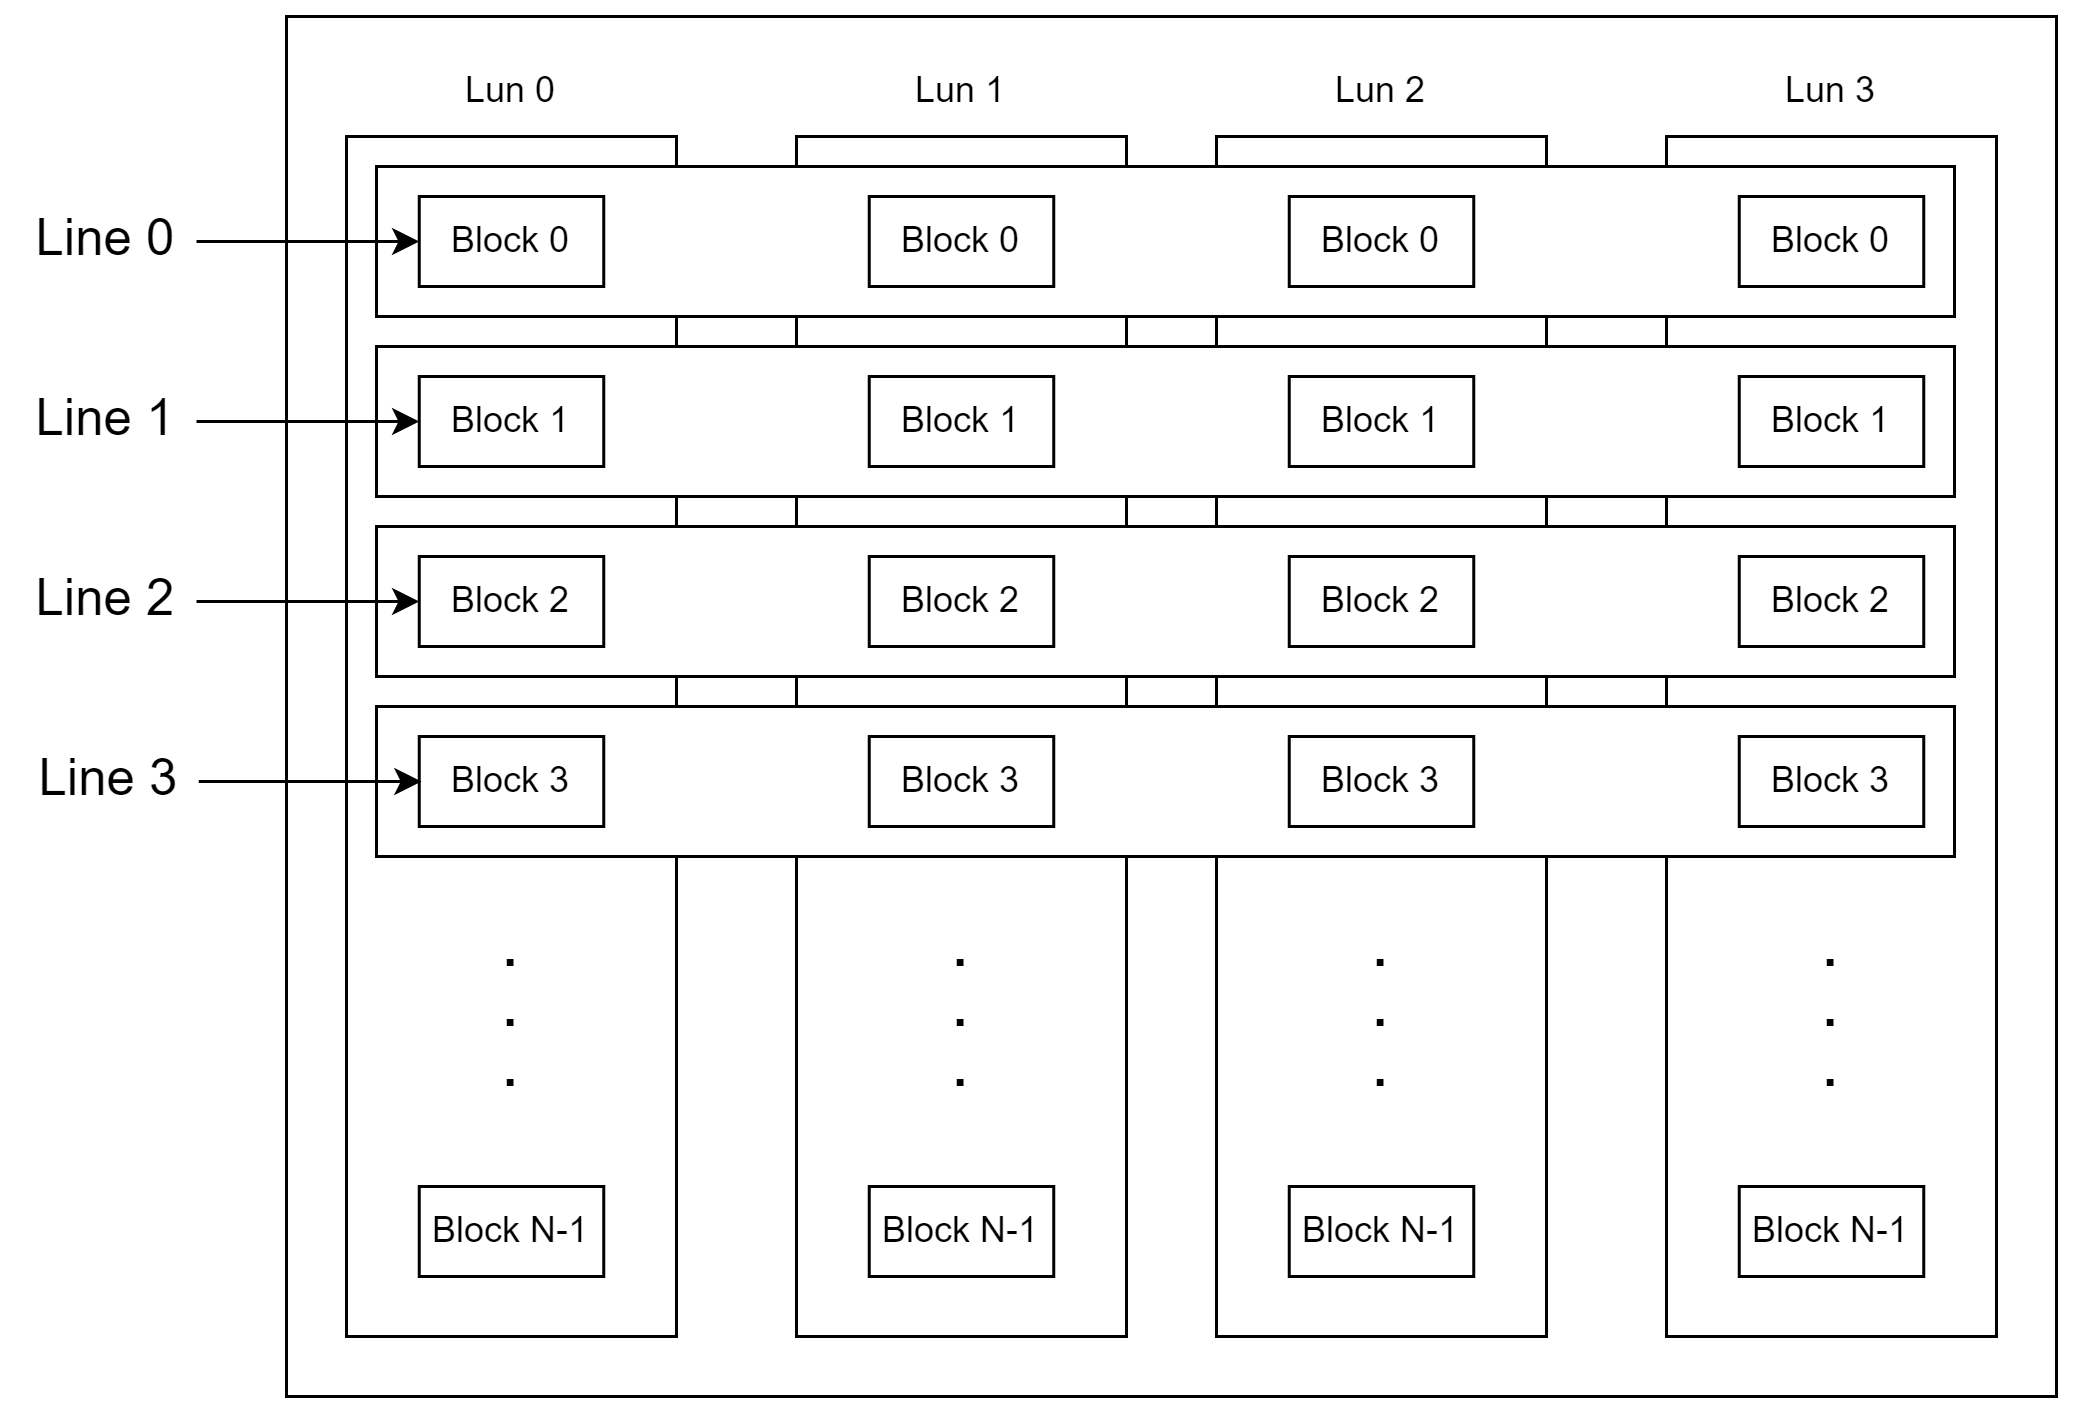
\includegraphics[width=1\textwidth]{picture/ch3/4Line.png}
    \caption{準備四個 Line}
    \label{f3.4}
\end{figure}

\newpage
\section{處理檔案系統要求之流程}\label{s3.2}
\indent
檔案系統提出 Request 要求之後,LightNVM 會對 Request 拆解,儲存成 LightNVM 自己容易處理的形式,但是在拆解的同時,會損失一些資訊,所以首先我們要先在拆解 Request 之前把 Request 的大小先從 Request 的資料結構 bio (Block I/O) \cite{10.1145/2619092}擷取出來,用大小來判斷這個 Request 的資料屬於哪一個分群,並將資訊塞入 LightNVM 用來儲存 Request 的地方 - Ring Buffer 之中,最後計算平均值,給下次 Request 傳進時使用。\cite{LightNVM}

\subsection{以平均值劃分熱門資料及冷門資料}\label{s3.2.1}
\indent
首先為了劃分熱門及冷門資料,我們將過去一萬筆 Request 大小的平均值當作基準,劃分四個等級,平均值的 0\% - 50\% 為最熱門的資料,平均值的 50\% - 100 \% 為第二熱門的資料,平均值的 100\% - 150\% 為第二冷門資料,平均值的 150\% 以上為最冷門的資料。並且由熱門到冷門所對應到的 Line 為 Line 0 到 Line 3(如圖\ref{f3.5}所示)。
\begin{figure}[H]
    \centering
    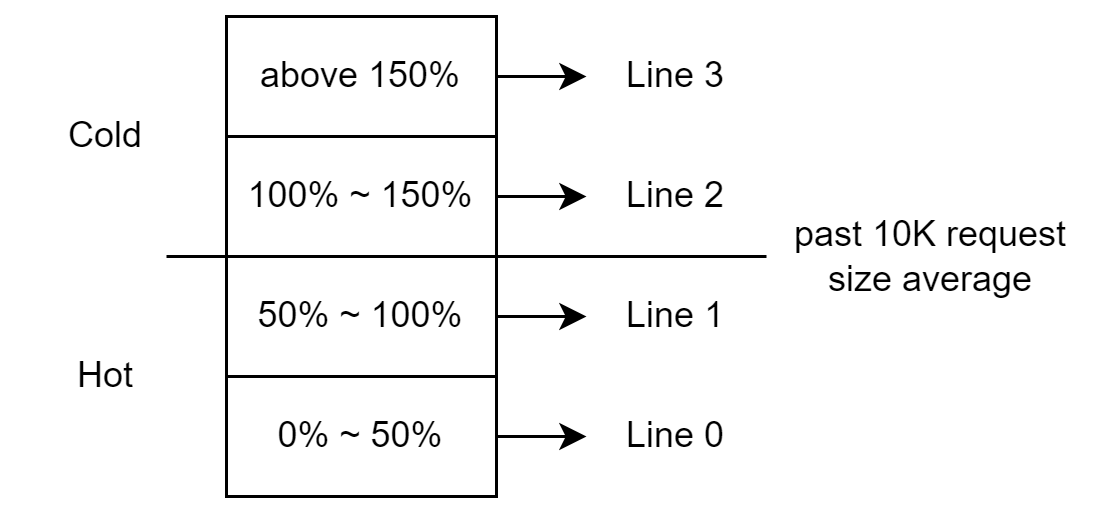
\includegraphics[width=0.8\textwidth]{picture/ch3/hot_cold.png}
    \caption{熱門資料與冷門資料}
    \label{f3.5}
\end{figure}

\subsection{擷取 Request 大小並判斷分群}\label{s3.2.2}
\indent
在得到 Request 大小時,我們需要從檔案系統傳給 LightNVM 的資料結構 bio 之中,找到 Request 大小的值;之後再以 Request 大小與平均值,判斷當下的 Request 屬於哪一類(如圖\ref{f3.6}所示)。
\begin{figure}[H]
    \centering
    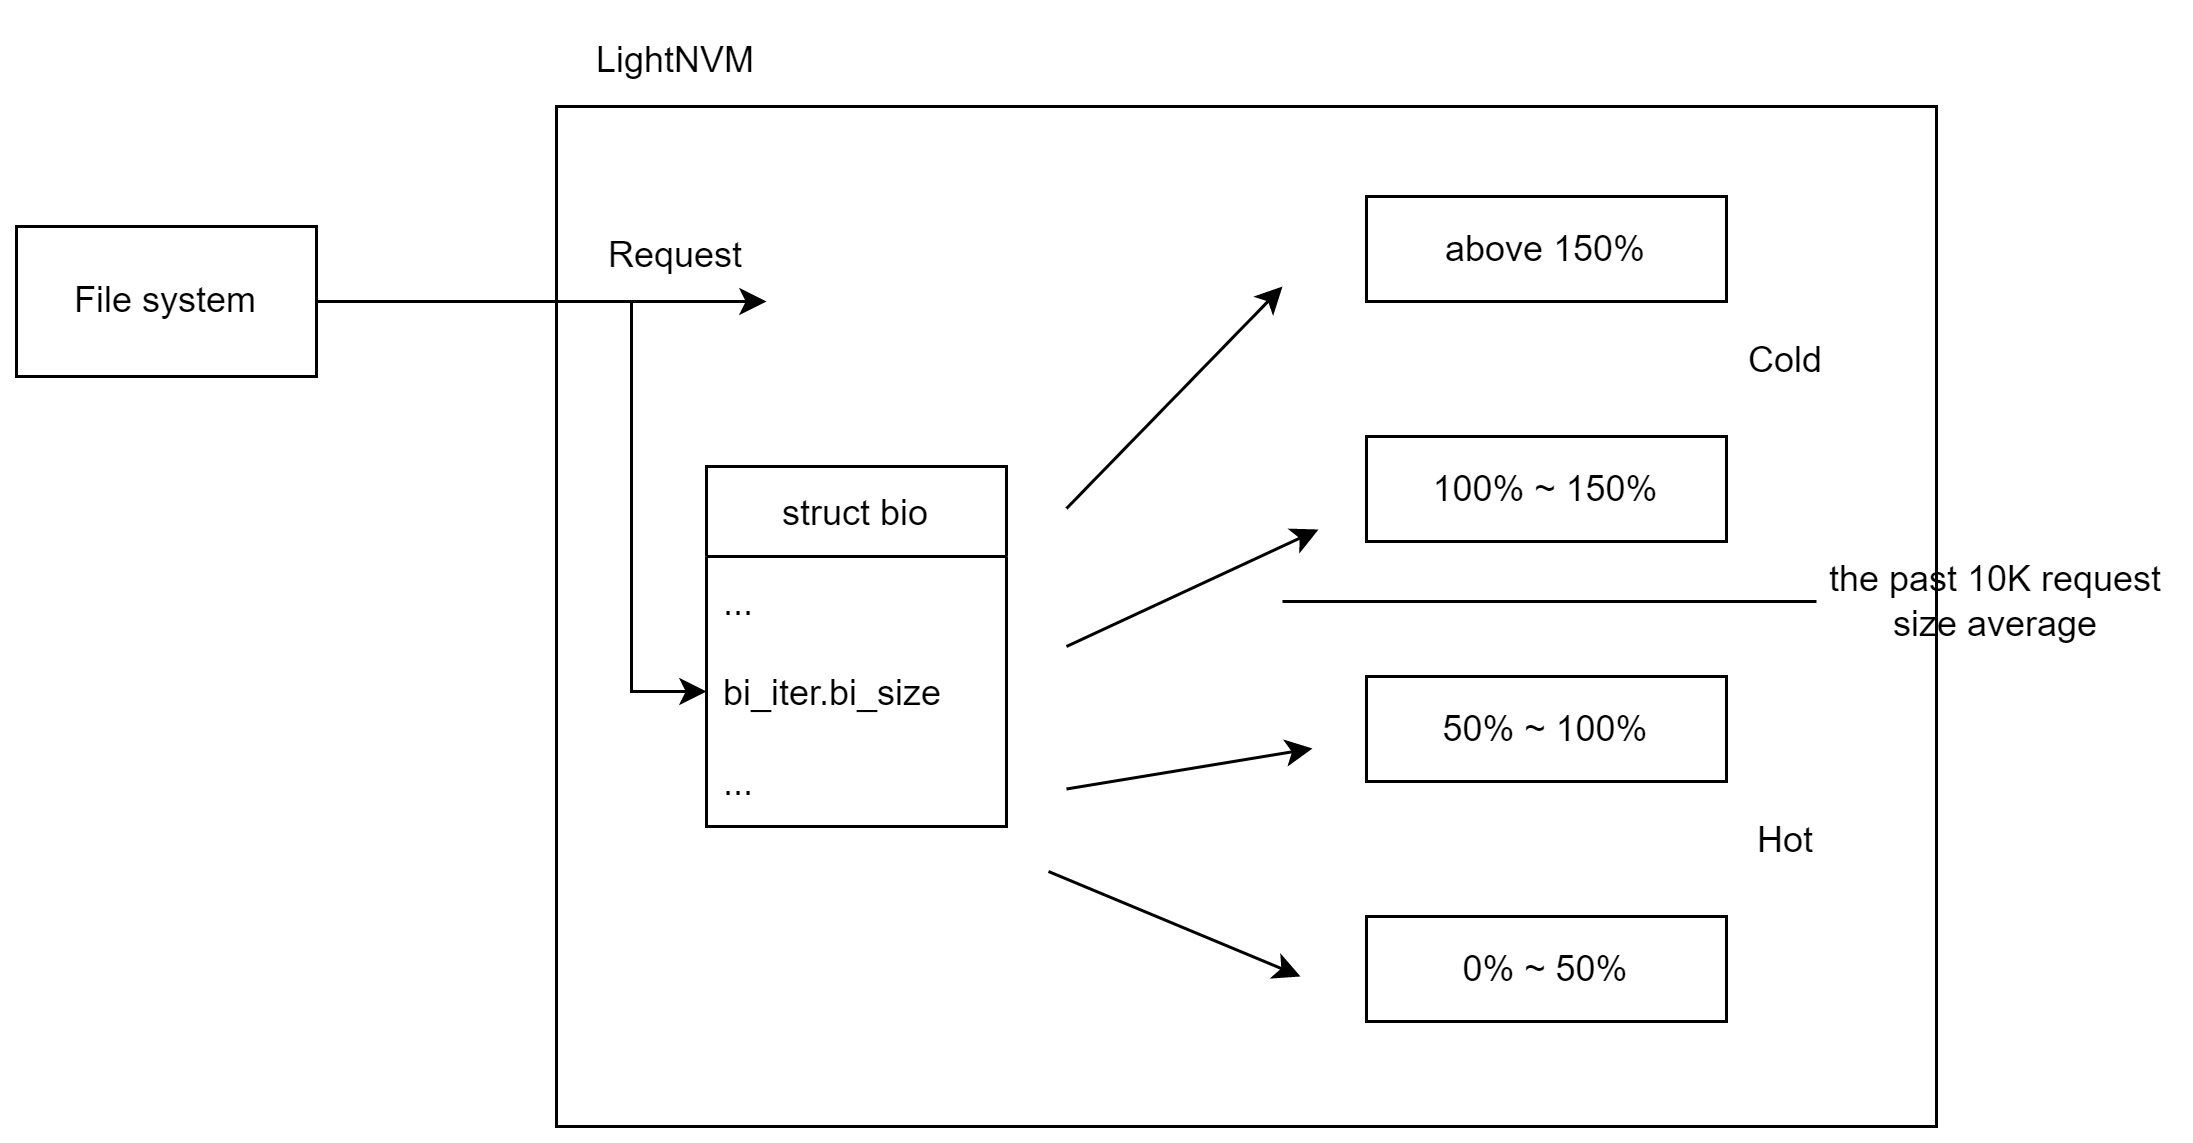
\includegraphics[width=1\textwidth]{picture/ch3/get_rq_size_hot_cold.png}
    \caption{判斷 Request 分群}
    \label{f3.6}
\end{figure}


\subsection{計算平均值}\label{s3.2.3}
\indent
在判斷完分群之後,我們需要拿剛剛得到的 Request 大小與平均值計算出新的平均值;由於我們需要前一萬筆 Request 大小的平均值,所以得到大小之後將其乘以 0.0001 倍再與我們加入 LightNVM 的平均值乘以 0.9999 倍之後相加,之後下一次檔案系統傳送 Request 進來時,就可以繼續用來判斷分群(如圖\ref{f3.7}所示)。
\begin{figure}[H]
    \centering
    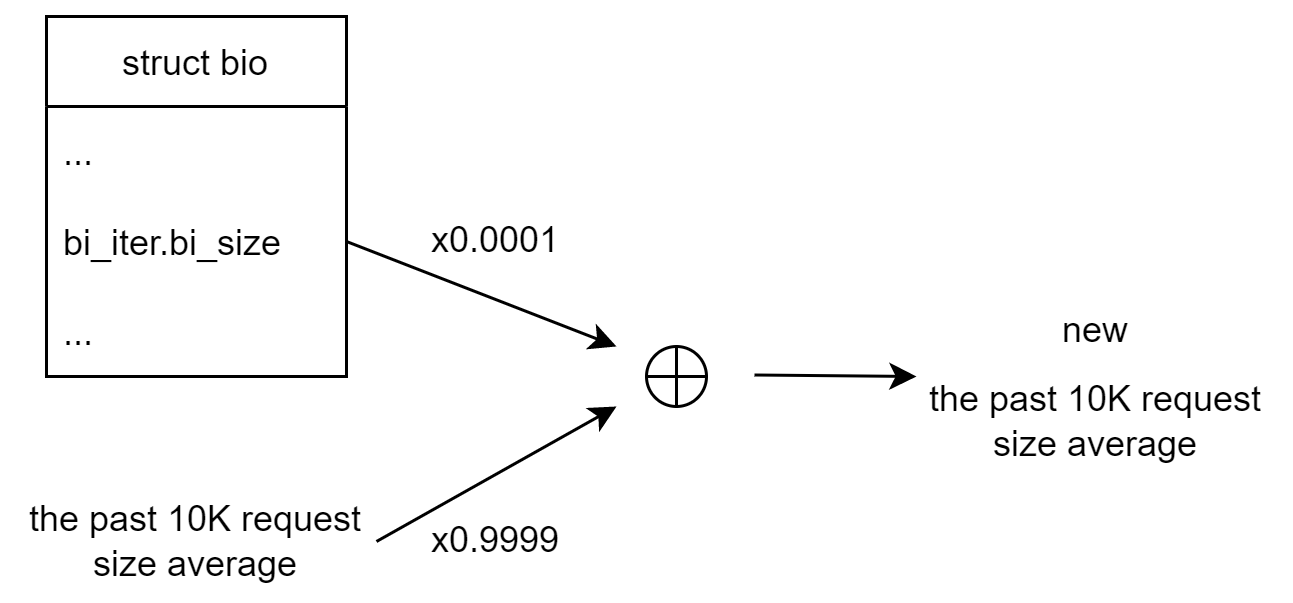
\includegraphics[width=0.8\textwidth]{picture/ch3/new_average.png}
    \caption{計算新平均值}
    \label{f3.7}
\end{figure}

\subsection{將 Request 所屬分群的資訊放入 Ring Buffer 中}\label{s3.2.4}
\indent
LightNVM 在接到檔案系統的 Request 之後,會將 Request 的資料拆解成數個 Page,每個 Page 都會記錄成 Ring Buffer 一個 Entry 之中,之後便會喚醒 LightNVM 背景的 write thread,從 Ring Buffer 存取剛剛放進去的 Entry,來得知寫入的資料位於 Host 記憶體,我們在這個 Entry 之中加入要存入哪個 Line,也就是冷熱分群的資訊,以便之後的 write thread 使用(如圖\ref{f3.8}所示)。

\begin{figure}[H]
    \centering
    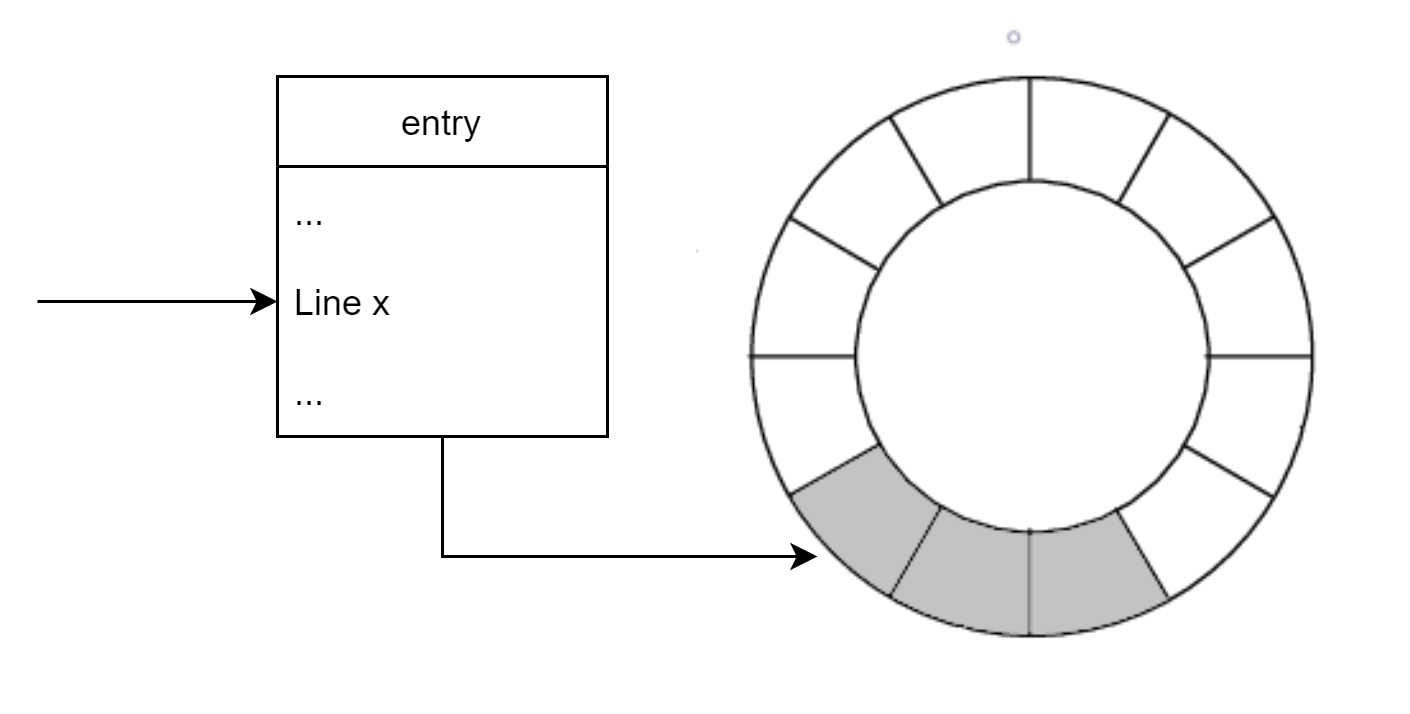
\includegraphics[width=0.7\textwidth]{picture/ch3/store_line_in_ring_buffer_entry.png}
    \caption{將分群資訊放入 Ring Buffer 的單位資料結構(Entry)}
    \label{f3.8}
\end{figure}

\section{實際寫入之過程}\label{s3.3}
\indent
LightNVM 的 Write Thread 被喚醒之後,會從剛剛紀錄到 Ring Buffer 之中的 Entry 得知要寫入的資料在哪裡,而我們也跟著得知剛剛我們放入的資訊,也就是每個 Entry 所屬的冷熱分群,接著我們將所有當次所提取的 Entry 的所屬冷熱分群總和之後取平均,得到的平均值就是我們最後寫入的 Line,最後我們將 Line 切換到我們的目標之後,LightNVM 就會根據我們所提供的 Line 來做 allocation,最終傳給 Open Channel SSD。

\subsection{從 Ring Buffer 中蒐集 Entry}\label{s3.3.1}
\indent
每次 LightNVM 從 Ring Buffer 之中抽取出的 Entry 數量不一定一樣,假設這次會取四個 Entry 的資料,分別所屬為 Line 3、2、1、2,那最後平均值是 2(如圖\ref{f3.9}所示)。

\begin{figure}[H]
    \centering
    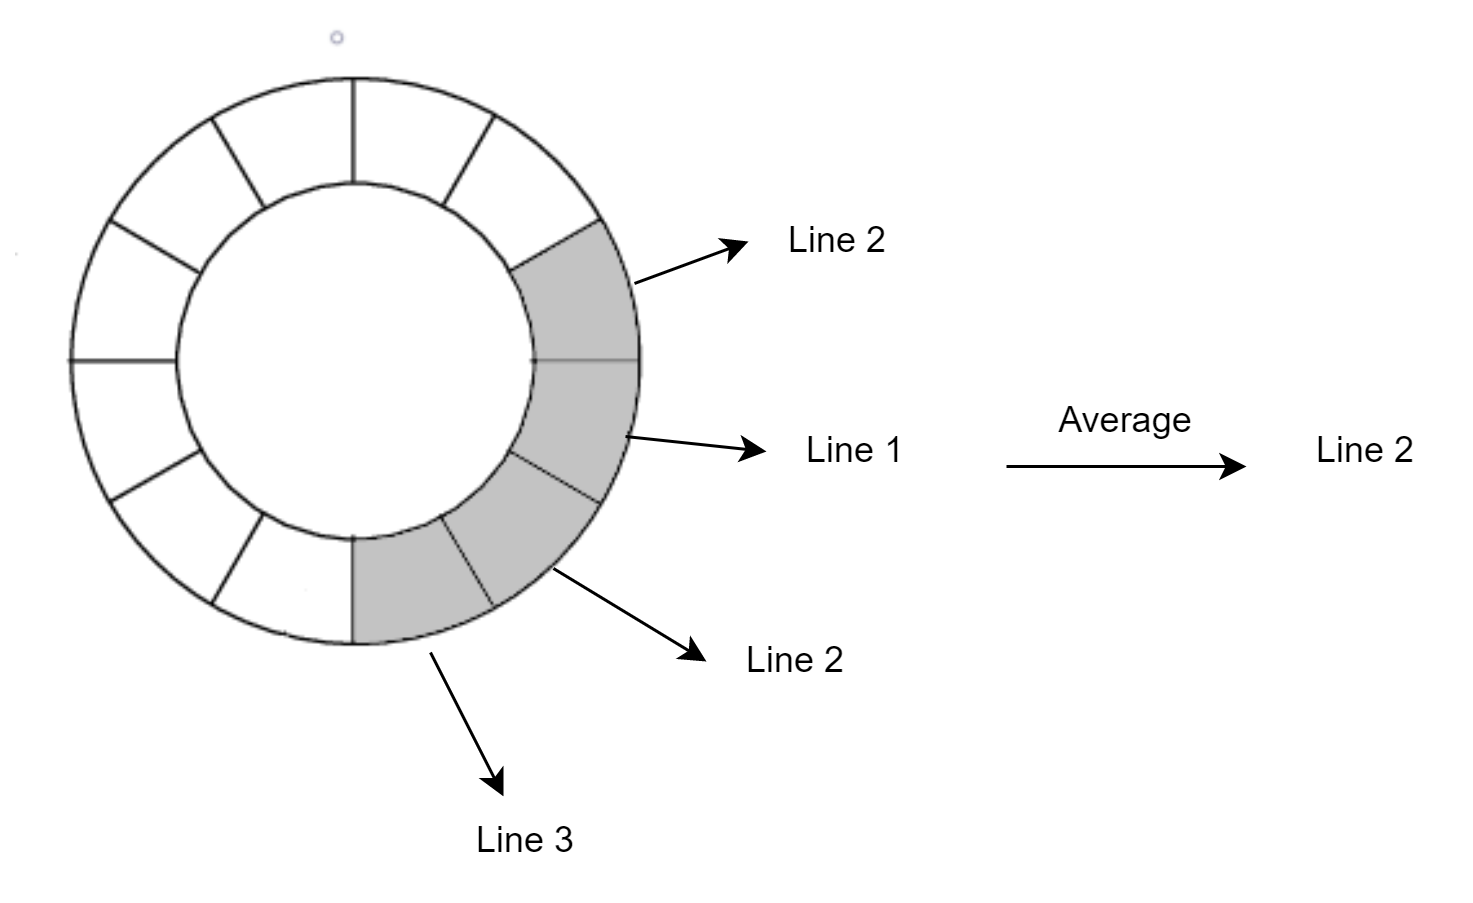
\includegraphics[width=0.7\textwidth]{picture/ch3/get_entry_from_ring_buffer.png}
    \caption{從數個 Entry 取出 Line 之後平均}
    \label{f3.9}
\end{figure}

\newpage
\subsection{切換 Line 之後傳送給 Open Channel SSD}\label{s3.3.2}
\indent
按照剛剛計算的平均值切換 Line 之後,LightNVM 會根據我們指定的 Line 做 Allocation,最後將資料以及位置往下傳給 Open Channel SSD(如圖\ref{f3.10}所示)(圖例延續 \ref{f3.9})。
\begin{figure}[H]
    \centering
    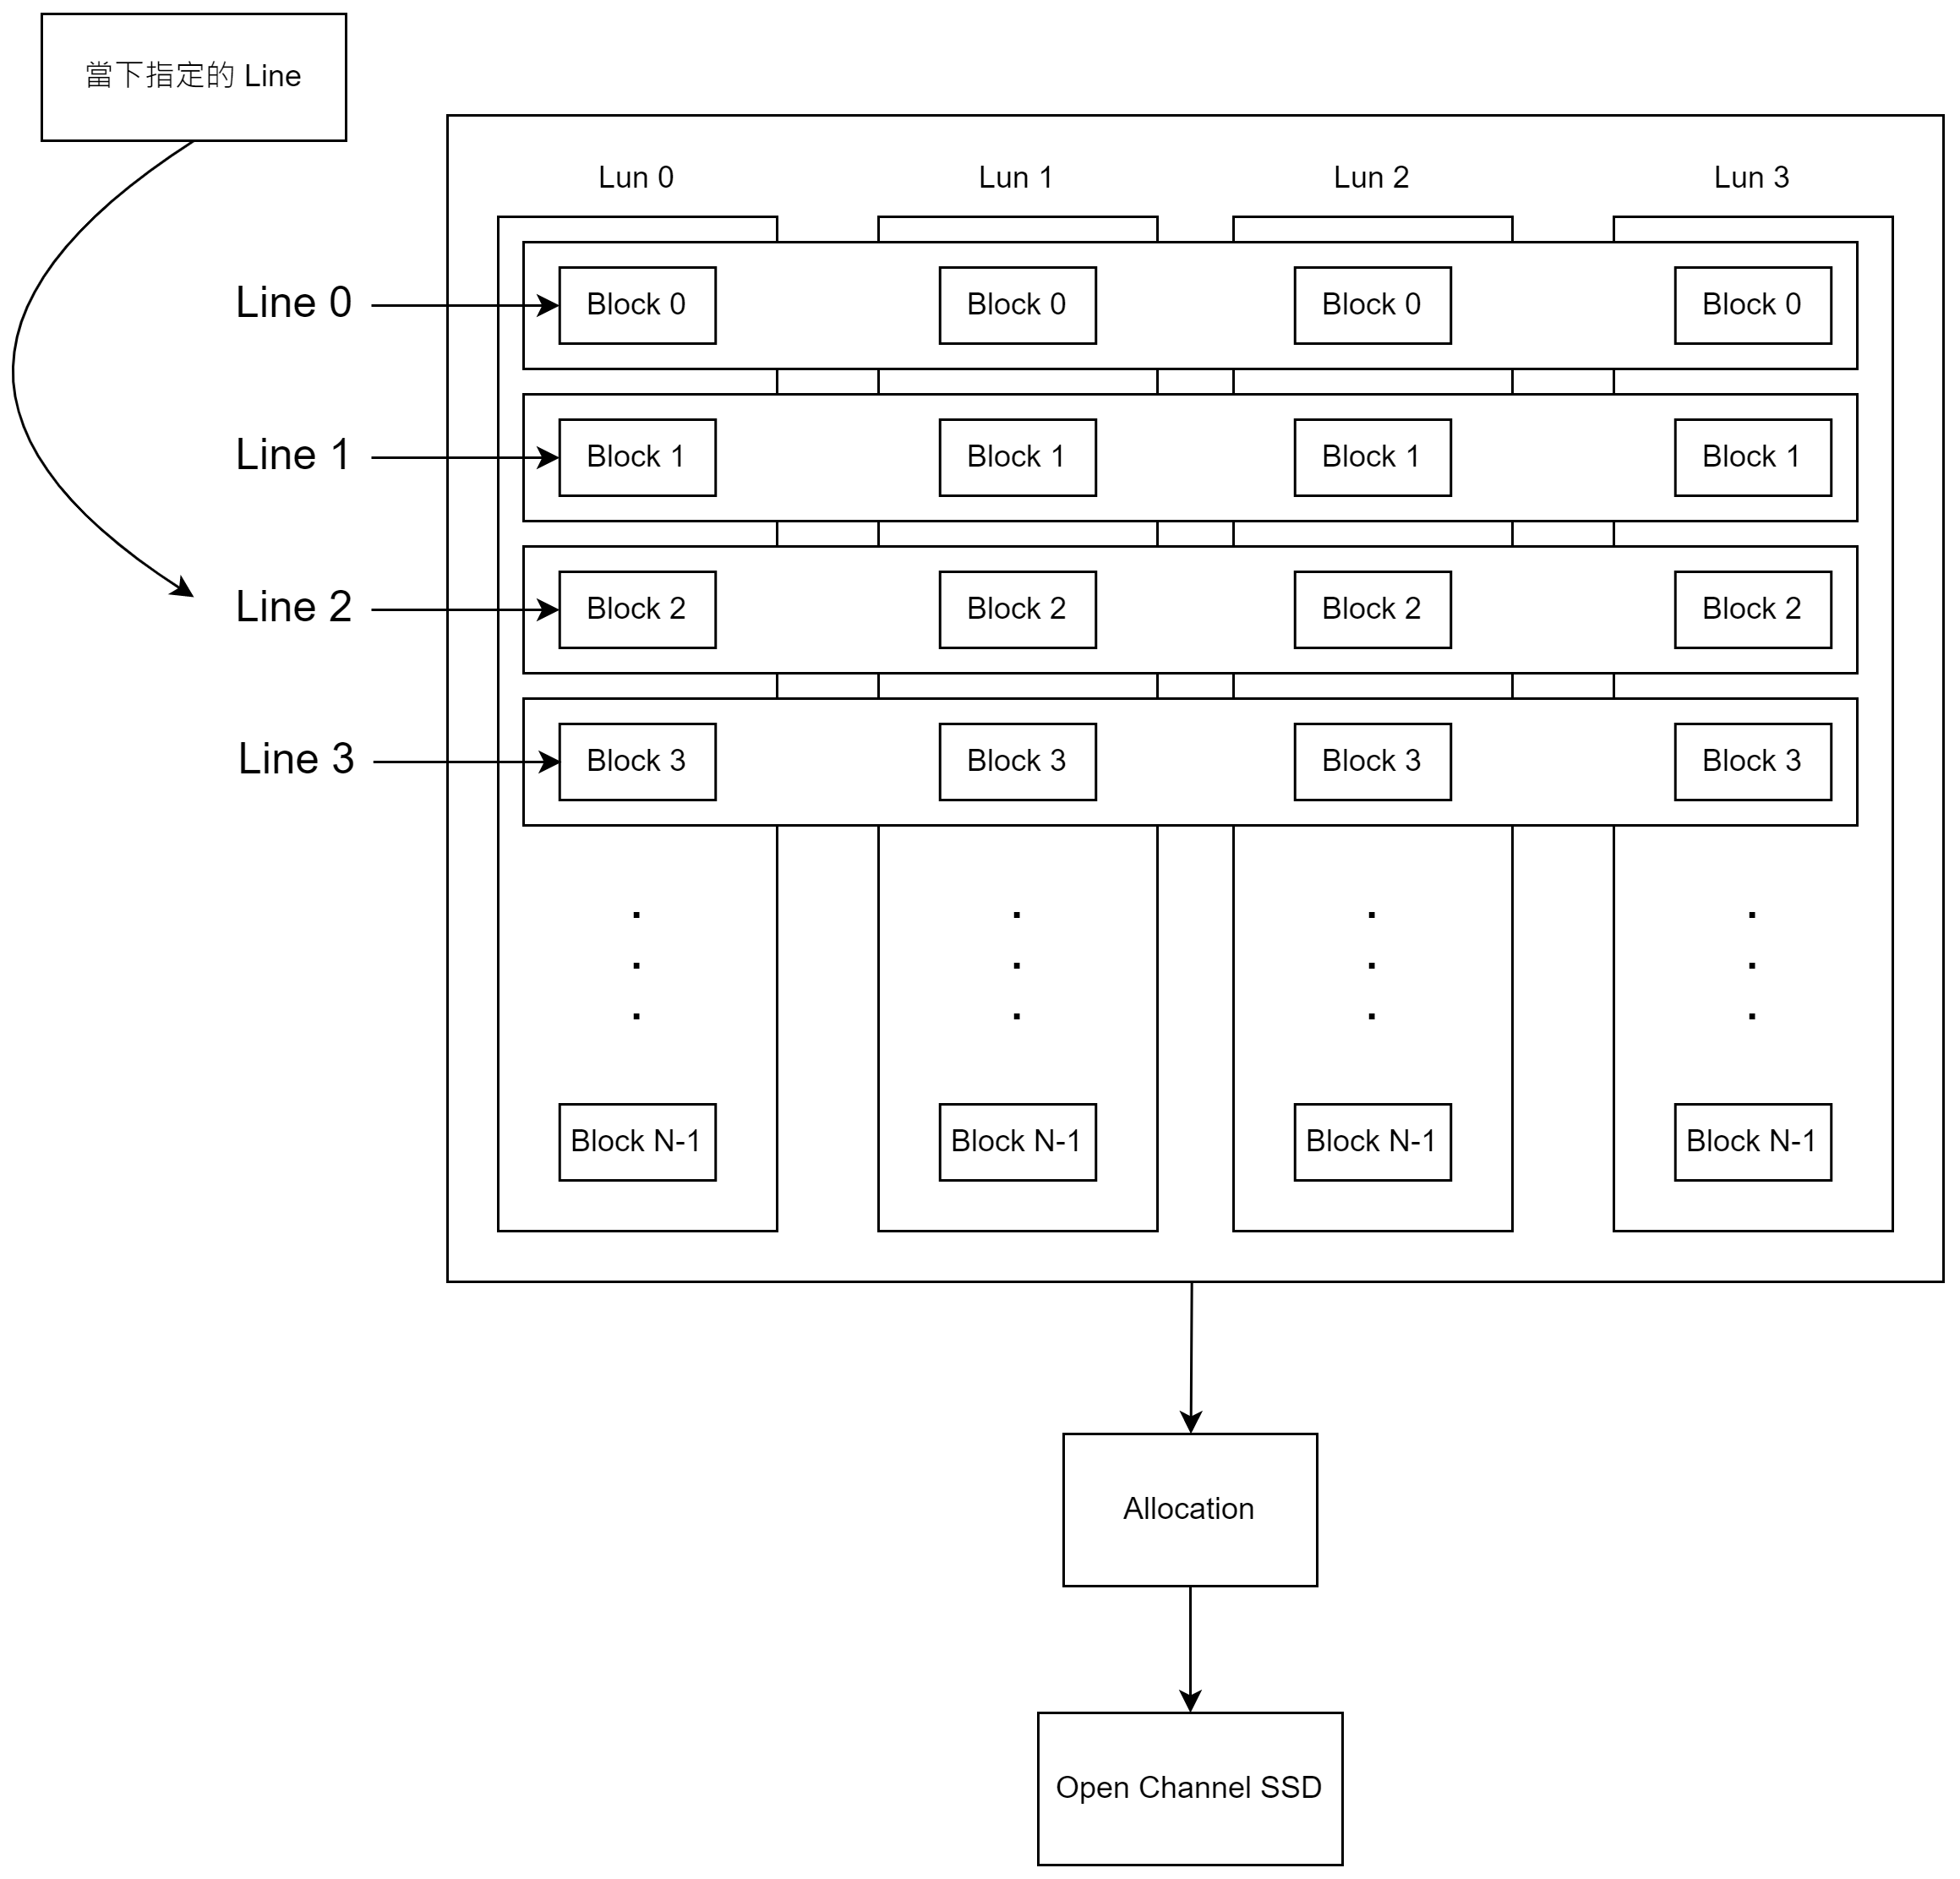
\includegraphics[width=1\textwidth]{picture/ch3/switch_line_to_opssd.drawio.png}
    \caption{切換 Line 之後 Allocation,最後傳給 Open Channel SSD}
    \label{f3.10}
\end{figure}